%-------------------------------------------------------------------------------
%                            BAB III
%               		METODOLOGI PENELITIAN
%-------------------------------------------------------------------------------
% \fancyhf{} 
% \fancyfoot[C]{\thepage}
\captionsetup[figure]{labelfont={normalfont}, textfont={normalfont}}

\chapter{METODOLOGI PENELITIAN}
%\usepackage{table,xcdraw}[xcolor]
%\thispagestyle{plain} % Halaman pertama bab menggunakan gaya plain

\section{Waktu dan Lokasi Penelitian}
Penelitian ini akan bertempat di Ruang Laboratorium Sistem Informasi dan Database di Lantai 3 Gedung A FMIPA USK. Pelaksanaan penelitian ini berlangsung selama enam bulan terhitung  dari bulan Januari 202X hingga Juni 202X. Jadwal pelaksanaan penelitian dapat dilihat pada Tabel \ref{tab:jadwal_pelaksanaan}.

% \section{Jadwal Pelaksanaan}

% \parUntuk lebih memahami alur waktu dari penelitian ini, penulis telah menyusun sebuah jadwal yang rinci yang bisa dilihat pada Tabel \ref{tab:jadwal_pelaksanaan}.


% \begin{table}[H]
%     \centering
%     \caption{Jadwal Pelaksanaan Penelitian}
%     \includegraphics[width=\textwidth]{image/bab3/jadwal-pelaksanaan.pdf}\label{tab:jadwal_pelaksanaan}
% \end{table}


% Please add the following required packages to your document preamble:
% \usepackage{multirow}
% \usepackage{graphicx}
% \usepackage[table,xcdraw]{xcolor}
% Beamer presentation requires \usepackage{colortbl} instead of \usepackage[table,xcdraw]{xcolor}
\begin{table}[H]
  \centering
  \caption{Jadwal pelaksanaan penelitian}
  \label{tab:jadwal_pelaksanaan}
  \resizebox{\textwidth}{!}{%
  \begin{tabular}{|l|l|llllllllllllllllllllllll|}
  \hline
   &
     &
    \multicolumn{24}{c|}{\textbf{Bulan Ke -}} \\ \cline{3-26} 
   &
     &
    \multicolumn{4}{c|}{\textbf{Januari}} &
    \multicolumn{4}{c|}{\textbf{Februari}} &
    \multicolumn{4}{c|}{\textbf{Maret}} &
    \multicolumn{4}{c|}{\textbf{April}} &
    \multicolumn{4}{c|}{\textbf{Mei}} &
    \multicolumn{4}{c|}{\textbf{Juni}} \\ \cline{3-26} 
  \multirow{-3}{*}{\textbf{No}} &
    \multirow{-3}{*}{\textbf{Kegiatan}} &
    \multicolumn{1}{c|}{\textbf{1}} &
    \multicolumn{1}{c|}{\textbf{2}} &
    \multicolumn{1}{c|}{\textbf{3}} &
    \multicolumn{1}{c|}{\textbf{4}} &
    \multicolumn{1}{c|}{\textbf{1}} &
    \multicolumn{1}{c|}{\textbf{2}} &
    \multicolumn{1}{c|}{\textbf{3}} &
    \multicolumn{1}{c|}{\textbf{4}} &
    \multicolumn{1}{c|}{\textbf{1}} &
    \multicolumn{1}{c|}{\textbf{2}} &
    \multicolumn{1}{c|}{\textbf{3}} &
    \multicolumn{1}{c|}{\textbf{4}} &
    \multicolumn{1}{c|}{\textbf{1}} &
    \multicolumn{1}{c|}{\textbf{2}} &
    \multicolumn{1}{c|}{\textbf{3}} &
    \multicolumn{1}{c|}{\textbf{4}} &
    \multicolumn{1}{c|}{\textbf{1}} &
    \multicolumn{1}{c|}{\textbf{2}} &
    \multicolumn{1}{c|}{\textbf{3}} &
    \multicolumn{1}{c|}{\textbf{4}} &
    \multicolumn{1}{c|}{\textbf{1}} &
    \multicolumn{1}{c|}{\textbf{2}} &
    \multicolumn{1}{c|}{\textbf{3}} &
    \multicolumn{1}{c|}{\textbf{4}} \\ \hline
  1 &
    Studi literatur &
    \multicolumn{1}{l|}{\cellcolor[HTML]{333333}{\color[HTML]{333333} }} &
    \multicolumn{1}{l|}{\cellcolor[HTML]{333333}{\color[HTML]{333333} }} &
    \multicolumn{1}{l|}{\cellcolor[HTML]{333333}{\color[HTML]{333333} }} &
    \multicolumn{1}{l|}{\cellcolor[HTML]{333333}{\color[HTML]{333333} }} &
    \multicolumn{1}{l|}{} &
    \multicolumn{1}{l|}{} &
    \multicolumn{1}{l|}{} &
    \multicolumn{1}{l|}{} &
    \multicolumn{1}{l|}{} &
    \multicolumn{1}{l|}{} &
    \multicolumn{1}{l|}{} &
    \multicolumn{1}{l|}{} &
    \multicolumn{1}{l|}{} &
    \multicolumn{1}{l|}{} &
    \multicolumn{1}{l|}{} &
    \multicolumn{1}{l|}{} &
    \multicolumn{1}{l|}{} &
    \multicolumn{1}{l|}{} &
    \multicolumn{1}{l|}{} &
    \multicolumn{1}{l|}{} &
    \multicolumn{1}{l|}{} &
    \multicolumn{1}{l|}{} &
    \multicolumn{1}{l|}{} &
     \\ \hline
  2 &
    Pengumpulan data &
    \multicolumn{1}{l|}{} &
    \multicolumn{1}{l|}{} &
    \multicolumn{1}{l|}{\cellcolor[HTML]{333333}} &
    \multicolumn{1}{l|}{\cellcolor[HTML]{333333}} &
    \multicolumn{1}{l|}{} &
    \multicolumn{1}{l|}{} &
    \multicolumn{1}{l|}{} &
    \multicolumn{1}{l|}{} &
    \multicolumn{1}{l|}{} &
    \multicolumn{1}{l|}{} &
    \multicolumn{1}{l|}{} &
    \multicolumn{1}{l|}{} &
    \multicolumn{1}{l|}{} &
    \multicolumn{1}{l|}{} &
    \multicolumn{1}{l|}{} &
    \multicolumn{1}{l|}{} &
    \multicolumn{1}{l|}{} &
    \multicolumn{1}{l|}{} &
    \multicolumn{1}{l|}{} &
    \multicolumn{1}{l|}{} &
    \multicolumn{1}{l|}{} &
    \multicolumn{1}{l|}{} &
    \multicolumn{1}{l|}{} &
     \\ \hline
  3 &
    Pra-pemrosesan data &
    \multicolumn{1}{l|}{} &
    \multicolumn{1}{l|}{} &
    \multicolumn{1}{l|}{} &
    \multicolumn{1}{l|}{} &
    \multicolumn{1}{l|}{\cellcolor[HTML]{333333}} &
    \multicolumn{1}{l|}{\cellcolor[HTML]{333333}} &
    \multicolumn{1}{l|}{\cellcolor[HTML]{333333}} &
    \multicolumn{1}{l|}{\cellcolor[HTML]{333333}} &
    \multicolumn{1}{l|}{\cellcolor[HTML]{333333}} &
    \multicolumn{1}{l|}{\cellcolor[HTML]{333333}} &
    \multicolumn{1}{l|}{} &
    \multicolumn{1}{l|}{} &
    \multicolumn{1}{l|}{} &
    \multicolumn{1}{l|}{} &
    \multicolumn{1}{l|}{} &
    \multicolumn{1}{l|}{} &
    \multicolumn{1}{l|}{} &
    \multicolumn{1}{l|}{} &
    \multicolumn{1}{l|}{} &
    \multicolumn{1}{l|}{} &
    \multicolumn{1}{l|}{} &
    \multicolumn{1}{l|}{} &
    \multicolumn{1}{l|}{} &
     \\ \hline
  4 &
    Pelatihan model &
    \multicolumn{1}{l|}{} &
    \multicolumn{1}{l|}{} &
    \multicolumn{1}{l|}{} &
    \multicolumn{1}{l|}{} &
    \multicolumn{1}{l|}{} &
    \multicolumn{1}{l|}{} &
    \multicolumn{1}{l|}{} &
    \multicolumn{1}{l|}{} &
    \multicolumn{1}{l|}{} &
    \multicolumn{1}{l|}{} &
    \multicolumn{1}{l|}{\cellcolor[HTML]{333333}} &
    \multicolumn{1}{l|}{\cellcolor[HTML]{333333}} &
    \multicolumn{1}{l|}{\cellcolor[HTML]{333333}} &
    \multicolumn{1}{l|}{\cellcolor[HTML]{333333}} &
    \multicolumn{1}{l|}{\cellcolor[HTML]{333333}} &
    \multicolumn{1}{l|}{\cellcolor[HTML]{333333}} &
    \multicolumn{1}{l|}{} &
    \multicolumn{1}{l|}{} &
    \multicolumn{1}{l|}{} &
    \multicolumn{1}{l|}{} &
    \multicolumn{1}{l|}{} &
    \multicolumn{1}{l|}{} &
    \multicolumn{1}{l|}{} &
     \\ \hline
  5 &
    evaluasi Model  &
    \multicolumn{1}{l|}{} &
    \multicolumn{1}{l|}{} &
    \multicolumn{1}{l|}{} &
    \multicolumn{1}{l|}{} &
    \multicolumn{1}{l|}{} &
    \multicolumn{1}{l|}{} &
    \multicolumn{1}{l|}{} &
    \multicolumn{1}{l|}{} &
    \multicolumn{1}{l|}{} &
    \multicolumn{1}{l|}{} &
    \multicolumn{1}{l|}{} &
    \multicolumn{1}{l|}{} &
    \multicolumn{1}{l|}{}&
    \multicolumn{1}{l|}{} &
    \multicolumn{1}{l|}{} &
    \multicolumn{1}{l|}{\cellcolor[HTML]{333333}} &
    \multicolumn{1}{l|}{\cellcolor[HTML]{333333}} &
    \multicolumn{1}{l|}{\cellcolor[HTML]{333333}} &
    \multicolumn{1}{l|}{} &
    \multicolumn{1}{l|}{} &
    \multicolumn{1}{l|}{} &
    \multicolumn{1}{l|}{} &
    \multicolumn{1}{l|}{} &
     \\ \hline
  6 &
    Analisis hasil &
    \multicolumn{1}{l|}{} &
    \multicolumn{1}{l|}{} &
    \multicolumn{1}{l|}{} &
    \multicolumn{1}{l|}{} &
    \multicolumn{1}{l|}{} &
    \multicolumn{1}{l|}{} &
    \multicolumn{1}{l|}{} &
    \multicolumn{1}{l|}{} &
    \multicolumn{1}{l|}{} &
    \multicolumn{1}{l|}{} &
    \multicolumn{1}{l|}{} &
    \multicolumn{1}{l|}{} &
    \multicolumn{1}{l|}{} &
    \multicolumn{1}{l|}{} &
    \multicolumn{1}{l|}{} &
    \multicolumn{1}{l|}{} &
    \multicolumn{1}{l|}{} &
    \multicolumn{1}{l|}{\cellcolor[HTML]{333333}} &
    \multicolumn{1}{l|}{\cellcolor[HTML]{333333}} &
    \multicolumn{1}{l|}{\cellcolor[HTML]{333333}} &
    \multicolumn{1}{l|}{} &
    \multicolumn{1}{l|}{} &
    \multicolumn{1}{l|}{} &
     \\ \hline
  7 &
    Penyusunan laporan akhir &
    \multicolumn{1}{l|}{} &
    \multicolumn{1}{l|}{} &
    \multicolumn{1}{l|}{} &
    \multicolumn{1}{l|}{} &
    \multicolumn{1}{l|}{} &
    \multicolumn{1}{l|}{} &
    \multicolumn{1}{l|}{} &
    \multicolumn{1}{l|}{} &
    \multicolumn{1}{l|}{} &
    \multicolumn{1}{l|}{} &
    \multicolumn{1}{l|}{} &
    \multicolumn{1}{l|}{} &
    \multicolumn{1}{l|}{} &
    \multicolumn{1}{l|}{} &
    \multicolumn{1}{l|}{} &
    \multicolumn{1}{l|}{} &
    \multicolumn{1}{l|}{} &
    \multicolumn{1}{l|}{} &
    \multicolumn{1}{l|}{} &
    \multicolumn{1}{l|}{\cellcolor[HTML]{333333}} &
    \multicolumn{1}{l|}{\cellcolor[HTML]{333333}} &
    \multicolumn{1}{l|}{\cellcolor[HTML]{333333}} &
    \multicolumn{1}{l|}{\cellcolor[HTML]{333333}} &
     \\ \hline
  \end{tabular}%
  }
  \end{table}


% Please add the following required packages to your document preamble:
% \usepackage{multirow}
% \usepackage{graphicx}
% \usepackage[table,xcdraw]{xcolor}
% Beamer presentation requires \usepackage{colortbl} instead of \usepackage[table,xcdraw]{xcolor}
% \begin{table}[H]
%     \centering
%     \caption{Jadwal pelaksanaan penelitian}
%     \label{tab: jadwal-pelaksanaan}
%     \resizebox{\textwidth}{!}{%
%     \begin{tabular}{|l|l|llll|llll|llll|llll|llll|llll|llll|llll|}
%     \hline
%      &
%        &
%       \multicolumn{4}{l|}{\textbf{November}} &
%       \multicolumn{4}{l|}{\textbf{Desember}} &
%       \multicolumn{4}{l|}{\textbf{Januari}} &
%       \multicolumn{4}{l|}{\textbf{Februari}} &
%       \multicolumn{4}{l|}{\textbf{Maret}} &
%       \multicolumn{4}{l|}{\textbf{April}} &
%       \multicolumn{4}{l|}{\textbf{Mei}} &
%       \multicolumn{4}{l|}{\textbf{Juni}} \\ \cline{3-34} 
%      &
%        &
%       \multicolumn{4}{l|}{\textbf{\begin{tabular}[c]{@{}l@{}}Minggu\\ Ke-\end{tabular}}} &
%       \multicolumn{4}{l|}{\textbf{\begin{tabular}[c]{@{}l@{}}Minggu\\ Ke-\end{tabular}}} &
%       \multicolumn{4}{l|}{\textbf{\begin{tabular}[c]{@{}l@{}}Minggu\\ Ke-\end{tabular}}} &
%       \multicolumn{4}{l|}{\textbf{\begin{tabular}[c]{@{}l@{}}Minggu\\ Ke-\end{tabular}}} &
%       \multicolumn{4}{l|}{\textbf{\begin{tabular}[c]{@{}l@{}}Minggu\\ Ke-\end{tabular}}} &
%       \multicolumn{4}{l|}{\textbf{\begin{tabular}[c]{@{}l@{}}Minggu\\ Ke-\end{tabular}}} &
%       \multicolumn{4}{l|}{\textbf{\begin{tabular}[c]{@{}l@{}}Minggu\\ Ke-\end{tabular}}} &
%       \multicolumn{4}{l|}{\textbf{\begin{tabular}[c]{@{}l@{}}Minggu\\ Ke-\end{tabular}}} \\ \cline{3-34} 
%     \multirow{-3}{*}{\textbf{No}} &
%       \multirow{-3}{*}{\textbf{Kegiatan}} &
%       \multicolumn{1}{l|}{\textbf{1}} &
%       \multicolumn{1}{l|}{\textbf{2}} &
%       \multicolumn{1}{l|}{\textbf{3}} &
%       \textbf{4} &
%       \multicolumn{1}{l|}{\textbf{1}} &
%       \multicolumn{1}{l|}{\textbf{2}} &
%       \multicolumn{1}{l|}{\textbf{3}} &
%       \textbf{4} &
%       \multicolumn{1}{l|}{\textbf{1}} &
%       \multicolumn{1}{l|}{\textbf{2}} &
%       \multicolumn{1}{l|}{\textbf{3}} &
%       \textbf{4} &
%       \multicolumn{1}{l|}{\textbf{1}} &
%       \multicolumn{1}{l|}{\textbf{2}} &
%       \multicolumn{1}{l|}{\textbf{3}} &
%       \textbf{4} &
%       \multicolumn{1}{l|}{\textbf{1}} &
%       \multicolumn{1}{l|}{\textbf{2}} &
%       \multicolumn{1}{l|}{\textbf{3}} &
%       \textbf{4} &
%       \multicolumn{1}{l|}{\textbf{1}} &
%       \multicolumn{1}{l|}{\textbf{2}} &
%       \multicolumn{1}{l|}{\textbf{3}} &
%       \textbf{4} &
%       \multicolumn{1}{l|}{\textbf{1}} &
%       \multicolumn{1}{l|}{\textbf{2}} &
%       \multicolumn{1}{l|}{\textbf{3}} &
%       \textbf{4} &
%       \multicolumn{1}{l|}{\textbf{1}} &
%       \multicolumn{1}{l|}{\textbf{2}} &
%       \multicolumn{1}{l|}{\textbf{3}} &
%       \textbf{4} \\ \hline
%     1 &
%       \begin{tabular}[c]{@{}l@{}}Pengajuan \\ Judul\end{tabular} &
%       \multicolumn{1}{l|}{\cellcolor[HTML]{666666}} &
%       \multicolumn{1}{l|}{\cellcolor[HTML]{666666}} &
%       \multicolumn{1}{l|}{} &
%        &
%       \multicolumn{1}{l|}{} &
%       \multicolumn{1}{l|}{} &
%       \multicolumn{1}{l|}{} &
%        &
%       \multicolumn{1}{l|}{} &
%       \multicolumn{1}{l|}{} &
%       \multicolumn{1}{l|}{} &
%        &
%       \multicolumn{1}{l|}{} &
%       \multicolumn{1}{l|}{} &
%       \multicolumn{1}{l|}{} &
%        &
%       \multicolumn{1}{l|}{} &
%       \multicolumn{1}{l|}{} &
%       \multicolumn{1}{l|}{} &
%        &
%       \multicolumn{1}{l|}{} &
%       \multicolumn{1}{l|}{} &
%       \multicolumn{1}{l|}{} &
%        &
%       \multicolumn{1}{l|}{} &
%       \multicolumn{1}{l|}{} &
%       \multicolumn{1}{l|}{} &
%        &
%       \multicolumn{1}{l|}{} &
%       \multicolumn{1}{l|}{} &
%       \multicolumn{1}{l|}{} &
%        \\ \hline
%     2 &
%       \begin{tabular}[c]{@{}l@{}}Studi \\ Literatur\end{tabular} &
%       \multicolumn{1}{l|}{\cellcolor[HTML]{666666}} &
%       \multicolumn{1}{l|}{\cellcolor[HTML]{666666}} &
%       \multicolumn{1}{l|}{} &
%        &
%       \multicolumn{1}{l|}{} &
%       \multicolumn{1}{l|}{} &
%       \multicolumn{1}{l|}{} &
%        &
%       \multicolumn{1}{l|}{} &
%       \multicolumn{1}{l|}{} &
%       \multicolumn{1}{l|}{} &
%        &
%       \multicolumn{1}{l|}{} &
%       \multicolumn{1}{l|}{} &
%       \multicolumn{1}{l|}{} &
%        &
%       \multicolumn{1}{l|}{} &
%       \multicolumn{1}{l|}{} &
%       \multicolumn{1}{l|}{} &
%        &
%       \multicolumn{1}{l|}{} &
%       \multicolumn{1}{l|}{} &
%       \multicolumn{1}{l|}{} &
%        &
%       \multicolumn{1}{l|}{} &
%       \multicolumn{1}{l|}{} &
%       \multicolumn{1}{l|}{} &
%        &
%       \multicolumn{1}{l|}{} &
%       \multicolumn{1}{l|}{} &
%       \multicolumn{1}{l|}{} &
%        \\ \hline
%     3 &
%       \begin{tabular}[c]{@{}l@{}}Penyusunan \\ BAB I\end{tabular} &
%       \multicolumn{1}{l|}{\cellcolor[HTML]{666666}} &
%       \multicolumn{1}{l|}{\cellcolor[HTML]{666666}} &
%       \multicolumn{1}{l|}{} &
%        &
%       \multicolumn{1}{l|}{} &
%       \multicolumn{1}{l|}{} &
%       \multicolumn{1}{l|}{} &
%        &
%       \multicolumn{1}{l|}{} &
%       \multicolumn{1}{l|}{} &
%       \multicolumn{1}{l|}{} &
%        &
%       \multicolumn{1}{l|}{} &
%       \multicolumn{1}{l|}{} &
%       \multicolumn{1}{l|}{} &
%        &
%       \multicolumn{1}{l|}{} &
%       \multicolumn{1}{l|}{} &
%       \multicolumn{1}{l|}{} &
%        &
%       \multicolumn{1}{l|}{} &
%       \multicolumn{1}{l|}{} &
%       \multicolumn{1}{l|}{} &
%        &
%       \multicolumn{1}{l|}{} &
%       \multicolumn{1}{l|}{} &
%       \multicolumn{1}{l|}{} &
%        &
%       \multicolumn{1}{l|}{} &
%       \multicolumn{1}{l|}{} &
%       \multicolumn{1}{l|}{} &
%        \\ \hline
%     4 &
%       \begin{tabular}[c]{@{}l@{}}Penyusunan \\ BAB II\end{tabular} &
%       \multicolumn{1}{l|}{} &
%       \multicolumn{1}{l|}{\cellcolor[HTML]{666666}} &
%       \multicolumn{1}{l|}{\cellcolor[HTML]{666666}} &
%       \cellcolor[HTML]{666666} &
%       \multicolumn{1}{l|}{\cellcolor[HTML]{666666}} &
%       \multicolumn{1}{l|}{} &
%       \multicolumn{1}{l|}{} &
%        &
%       \multicolumn{1}{l|}{} &
%       \multicolumn{1}{l|}{} &
%       \multicolumn{1}{l|}{} &
%        &
%       \multicolumn{1}{l|}{} &
%       \multicolumn{1}{l|}{} &
%       \multicolumn{1}{l|}{} &
%        &
%       \multicolumn{1}{l|}{} &
%       \multicolumn{1}{l|}{} &
%       \multicolumn{1}{l|}{} &
%        &
%       \multicolumn{1}{l|}{} &
%       \multicolumn{1}{l|}{} &
%       \multicolumn{1}{l|}{} &
%        &
%       \multicolumn{1}{l|}{} &
%       \multicolumn{1}{l|}{} &
%       \multicolumn{1}{l|}{} &
%        &
%       \multicolumn{1}{l|}{} &
%       \multicolumn{1}{l|}{} &
%       \multicolumn{1}{l|}{} &
%        \\ \hline
%     5 &
%       \begin{tabular}[c]{@{}l@{}}Penyusunan \\ BAB III\end{tabular} &
%       \multicolumn{1}{l|}{} &
%       \multicolumn{1}{l|}{} &
%       \multicolumn{1}{l|}{\cellcolor[HTML]{666666}} &
%       \cellcolor[HTML]{666666} &
%       \multicolumn{1}{l|}{\cellcolor[HTML]{666666}} &
%       \multicolumn{1}{l|}{\cellcolor[HTML]{666666}} &
%       \multicolumn{1}{l|}{\cellcolor[HTML]{666666}} &
%       \cellcolor[HTML]{666666} &
%       \multicolumn{1}{l|}{} &
%       \multicolumn{1}{l|}{} &
%       \multicolumn{1}{l|}{} &
%        &
%       \multicolumn{1}{l|}{} &
%       \multicolumn{1}{l|}{} &
%       \multicolumn{1}{l|}{} &
%        &
%       \multicolumn{1}{l|}{} &
%       \multicolumn{1}{l|}{} &
%       \multicolumn{1}{l|}{} &
%        &
%       \multicolumn{1}{l|}{} &
%       \multicolumn{1}{l|}{} &
%       \multicolumn{1}{l|}{} &
%        &
%       \multicolumn{1}{l|}{} &
%       \multicolumn{1}{l|}{} &
%       \multicolumn{1}{l|}{} &
%        &
%       \multicolumn{1}{l|}{} &
%       \multicolumn{1}{l|}{} &
%       \multicolumn{1}{l|}{} &
%        \\ \hline
%     6 &
%       \begin{tabular}[c]{@{}l@{}}Proposal \\ ACC\end{tabular} &
%       \multicolumn{1}{l|}{} &
%       \multicolumn{1}{l|}{} &
%       \multicolumn{1}{l|}{} &
%        &
%       \multicolumn{1}{l|}{} &
%       \multicolumn{1}{l|}{} &
%       \multicolumn{1}{l|}{} &
%        &
%       \multicolumn{1}{l|}{\cellcolor[HTML]{666666}} &
%       \multicolumn{1}{l|}{} &
%       \multicolumn{1}{l|}{} &
%        &
%       \multicolumn{1}{l|}{} &
%       \multicolumn{1}{l|}{} &
%       \multicolumn{1}{l|}{} &
%        &
%       \multicolumn{1}{l|}{} &
%       \multicolumn{1}{l|}{} &
%       \multicolumn{1}{l|}{} &
%        &
%       \multicolumn{1}{l|}{} &
%       \multicolumn{1}{l|}{} &
%       \multicolumn{1}{l|}{} &
%        &
%       \multicolumn{1}{l|}{} &
%       \multicolumn{1}{l|}{} &
%       \multicolumn{1}{l|}{} &
%        &
%       \multicolumn{1}{l|}{} &
%       \multicolumn{1}{l|}{} &
%       \multicolumn{1}{l|}{} &
%        \\ \hline
%     7 &
%       \begin{tabular}[c]{@{}l@{}}Seminar \\ Proposal\end{tabular} &
%       \multicolumn{1}{l|}{} &
%       \multicolumn{1}{l|}{} &
%       \multicolumn{1}{l|}{} &
%        &
%       \multicolumn{1}{l|}{} &
%       \multicolumn{1}{l|}{} &
%       \multicolumn{1}{l|}{} &
%        &
%       \multicolumn{1}{l|}{} &
%       \multicolumn{1}{l|}{\cellcolor[HTML]{666666}} &
%       \multicolumn{1}{l|}{} &
%        &
%       \multicolumn{1}{l|}{} &
%       \multicolumn{1}{l|}{} &
%       \multicolumn{1}{l|}{} &
%        &
%       \multicolumn{1}{l|}{} &
%       \multicolumn{1}{l|}{} &
%       \multicolumn{1}{l|}{} &
%        &
%       \multicolumn{1}{l|}{} &
%       \multicolumn{1}{l|}{} &
%       \multicolumn{1}{l|}{} &
%        &
%       \multicolumn{1}{l|}{} &
%       \multicolumn{1}{l|}{} &
%       \multicolumn{1}{l|}{} &
%        &
%       \multicolumn{1}{l|}{} &
%       \multicolumn{1}{l|}{} &
%       \multicolumn{1}{l|}{} &
%        \\ \hline
%     8 &
%       \begin{tabular}[c]{@{}l@{}}Revisi \\ Seminar \\ Proposal\end{tabular} &
%       \multicolumn{1}{l|}{} &
%       \multicolumn{1}{l|}{} &
%       \multicolumn{1}{l|}{} &
%        &
%       \multicolumn{1}{l|}{} &
%       \multicolumn{1}{l|}{} &
%       \multicolumn{1}{l|}{} &
%        &
%       \multicolumn{1}{l|}{} &
%       \multicolumn{1}{l|}{} &
%       \multicolumn{1}{l|}{\cellcolor[HTML]{666666}} &
%       \cellcolor[HTML]{666666} &
%       \multicolumn{1}{l|}{\cellcolor[HTML]{666666}} &
%       \multicolumn{1}{l|}{\cellcolor[HTML]{666666}} &
%       \multicolumn{1}{l|}{} &
%        &
%       \multicolumn{1}{l|}{} &
%       \multicolumn{1}{l|}{} &
%       \multicolumn{1}{l|}{} &
%        &
%       \multicolumn{1}{l|}{} &
%       \multicolumn{1}{l|}{} &
%       \multicolumn{1}{l|}{} &
%        &
%       \multicolumn{1}{l|}{} &
%       \multicolumn{1}{l|}{} &
%       \multicolumn{1}{l|}{} &
%        &
%       \multicolumn{1}{l|}{} &
%       \multicolumn{1}{l|}{} &
%       \multicolumn{1}{l|}{} &
%        \\ \hline
%     9 &
%       \begin{tabular}[c]{@{}l@{}}Pelaksanaan \\ Penelitian\end{tabular} &
%       \multicolumn{1}{l|}{} &
%       \multicolumn{1}{l|}{} &
%       \multicolumn{1}{l|}{} &
%        &
%       \multicolumn{1}{l|}{} &
%       \multicolumn{1}{l|}{} &
%       \multicolumn{1}{l|}{} &
%        &
%       \multicolumn{1}{l|}{} &
%       \multicolumn{1}{l|}{} &
%       \multicolumn{1}{l|}{\cellcolor[HTML]{666666}} &
%       \cellcolor[HTML]{666666} &
%       \multicolumn{1}{l|}{\cellcolor[HTML]{666666}} &
%       \multicolumn{1}{l|}{\cellcolor[HTML]{666666}} &
%       \multicolumn{1}{l|}{\cellcolor[HTML]{666666}} &
%       \cellcolor[HTML]{666666} &
%       \multicolumn{1}{l|}{\cellcolor[HTML]{666666}} &
%       \multicolumn{1}{l|}{\cellcolor[HTML]{666666}} &
%       \multicolumn{1}{l|}{\cellcolor[HTML]{666666}} &
%       \cellcolor[HTML]{666666} &
%       \multicolumn{1}{l|}{\cellcolor[HTML]{666666}} &
%       \multicolumn{1}{l|}{\cellcolor[HTML]{666666}} &
%       \multicolumn{1}{l|}{\cellcolor[HTML]{666666}} &
%       \cellcolor[HTML]{666666} &
%       \multicolumn{1}{l|}{\cellcolor[HTML]{666666}} &
%       \multicolumn{1}{l|}{} &
%       \multicolumn{1}{l|}{} &
%        &
%       \multicolumn{1}{l|}{} &
%       \multicolumn{1}{l|}{} &
%       \multicolumn{1}{l|}{} &
%        \\ \hline
%     10 &
%       \begin{tabular}[c]{@{}l@{}}Penyusuan \\ BAB IV\end{tabular} &
%       \multicolumn{1}{l|}{} &
%       \multicolumn{1}{l|}{} &
%       \multicolumn{1}{l|}{} &
%        &
%       \multicolumn{1}{l|}{} &
%       \multicolumn{1}{l|}{} &
%       \multicolumn{1}{l|}{} &
%        &
%       \multicolumn{1}{l|}{} &
%       \multicolumn{1}{l|}{} &
%       \multicolumn{1}{l|}{} &
%        &
%       \multicolumn{1}{l|}{} &
%       \multicolumn{1}{l|}{} &
%       \multicolumn{1}{l|}{} &
%        &
%       \multicolumn{1}{l|}{} &
%       \multicolumn{1}{l|}{} &
%       \multicolumn{1}{l|}{} &
%        &
%       \multicolumn{1}{l|}{} &
%       \multicolumn{1}{l|}{} &
%       \multicolumn{1}{l|}{} &
%       \cellcolor[HTML]{666666} &
%       \multicolumn{1}{l|}{\cellcolor[HTML]{666666}} &
%       \multicolumn{1}{l|}{\cellcolor[HTML]{666666}} &
%       \multicolumn{1}{l|}{\cellcolor[HTML]{666666}} &
%       \cellcolor[HTML]{666666} &
%       \multicolumn{1}{l|}{} &
%       \multicolumn{1}{l|}{} &
%       \multicolumn{1}{l|}{} &
%        \\ \hline
%     11 &
%       \begin{tabular}[c]{@{}l@{}}Penyusunan \\ BAB V\end{tabular} &
%       \multicolumn{1}{l|}{} &
%       \multicolumn{1}{l|}{} &
%       \multicolumn{1}{l|}{} &
%        &
%       \multicolumn{1}{l|}{} &
%       \multicolumn{1}{l|}{} &
%       \multicolumn{1}{l|}{} &
%        &
%       \multicolumn{1}{l|}{} &
%       \multicolumn{1}{l|}{} &
%       \multicolumn{1}{l|}{} &
%        &
%       \multicolumn{1}{l|}{} &
%       \multicolumn{1}{l|}{} &
%       \multicolumn{1}{l|}{} &
%        &
%       \multicolumn{1}{l|}{} &
%       \multicolumn{1}{l|}{} &
%       \multicolumn{1}{l|}{} &
%        &
%       \multicolumn{1}{l|}{} &
%       \multicolumn{1}{l|}{} &
%       \multicolumn{1}{l|}{} &
%        &
%       \multicolumn{1}{l|}{} &
%       \multicolumn{1}{l|}{} &
%       \multicolumn{1}{l|}{\cellcolor[HTML]{666666}} &
%       \cellcolor[HTML]{666666} &
%       \multicolumn{1}{l|}{} &
%       \multicolumn{1}{l|}{} &
%       \multicolumn{1}{l|}{} &
%        \\ \hline
%     12 &
%       \begin{tabular}[c]{@{}l@{}}Seminar\\ Hasil\end{tabular} &
%       \multicolumn{1}{l|}{} &
%       \multicolumn{1}{l|}{} &
%       \multicolumn{1}{l|}{} &
%        &
%       \multicolumn{1}{l|}{} &
%       \multicolumn{1}{l|}{} &
%       \multicolumn{1}{l|}{} &
%        &
%       \multicolumn{1}{l|}{} &
%       \multicolumn{1}{l|}{} &
%       \multicolumn{1}{l|}{} &
%        &
%       \multicolumn{1}{l|}{} &
%       \multicolumn{1}{l|}{} &
%       \multicolumn{1}{l|}{} &
%        &
%       \multicolumn{1}{l|}{} &
%       \multicolumn{1}{l|}{} &
%       \multicolumn{1}{l|}{} &
%        &
%       \multicolumn{1}{l|}{} &
%       \multicolumn{1}{l|}{} &
%       \multicolumn{1}{l|}{} &
%        &
%       \multicolumn{1}{l|}{} &
%       \multicolumn{1}{l|}{} &
%       \multicolumn{1}{l|}{} &
%        &
%       \multicolumn{1}{l|}{\cellcolor[HTML]{666666}} &
%       \multicolumn{1}{l|}{} &
%       \multicolumn{1}{l|}{} &
%        \\ \hline
%     13 &
%       \begin{tabular}[c]{@{}l@{}}Revisi \\ Seminar \\ Hasil\end{tabular} &
%       \multicolumn{1}{l|}{} &
%       \multicolumn{1}{l|}{} &
%       \multicolumn{1}{l|}{} &
%        &
%       \multicolumn{1}{l|}{} &
%       \multicolumn{1}{l|}{} &
%       \multicolumn{1}{l|}{} &
%        &
%       \multicolumn{1}{l|}{} &
%       \multicolumn{1}{l|}{} &
%       \multicolumn{1}{l|}{} &
%        &
%       \multicolumn{1}{l|}{} &
%       \multicolumn{1}{l|}{} &
%       \multicolumn{1}{l|}{} &
%        &
%       \multicolumn{1}{l|}{} &
%       \multicolumn{1}{l|}{} &
%       \multicolumn{1}{l|}{} &
%        &
%       \multicolumn{1}{l|}{} &
%       \multicolumn{1}{l|}{} &
%       \multicolumn{1}{l|}{} &
%        &
%       \multicolumn{1}{l|}{} &
%       \multicolumn{1}{l|}{} &
%       \multicolumn{1}{l|}{} &
%        &
%       \multicolumn{1}{l|}{\cellcolor[HTML]{666666}} &
%       \multicolumn{1}{l|}{\cellcolor[HTML]{666666}} &
%       \multicolumn{1}{l|}{} &
%        \\ \hline
%     14 &
%       Sidang &
%       \multicolumn{1}{l|}{} &
%       \multicolumn{1}{l|}{} &
%       \multicolumn{1}{l|}{} &
%        &
%       \multicolumn{1}{l|}{} &
%       \multicolumn{1}{l|}{} &
%       \multicolumn{1}{l|}{} &
%        &
%       \multicolumn{1}{l|}{} &
%       \multicolumn{1}{l|}{} &
%       \multicolumn{1}{l|}{} &
%        &
%       \multicolumn{1}{l|}{} &
%       \multicolumn{1}{l|}{} &
%       \multicolumn{1}{l|}{} &
%        &
%       \multicolumn{1}{l|}{} &
%       \multicolumn{1}{l|}{} &
%       \multicolumn{1}{l|}{} &
%        &
%       \multicolumn{1}{l|}{} &
%       \multicolumn{1}{l|}{} &
%       \multicolumn{1}{l|}{} &
%        &
%       \multicolumn{1}{l|}{} &
%       \multicolumn{1}{l|}{} &
%       \multicolumn{1}{l|}{} &
%        &
%       \multicolumn{1}{l|}{} &
%       \multicolumn{1}{l|}{} &
%       \multicolumn{1}{l|}{} &
%       \cellcolor[HTML]{666666} \\ \hline
%     \end{tabular}%
%     }
% \end{table}

\section{Alat dan Bahan}
\par Penelitian ini menggunakan perangkat keras dan perangkat lunak sebagai alat bantu dalam proses pengembangan dan implementasi algoritma \textit{K-Nearest Neighbors} (KNN). Perangkat keras digunakan untuk menjalankan simulasi dan pelatihan model, sedangkan perangkat lunak digunakan untuk pemrosesan data, pembuatan model, serta evaluasi performa. 

\subsection{Perangkat keras} % sesuaikan spec dari perangkat
\par Perangkat keras yang digunakan dalam penelitian ini adalah Laptop prosesor Intel Core i7, RAM 8 GB Penyimpanan, SSD minimal 512 GB, dan sistem Operasi Linux (Ubuntu 20.04+)

\subsection{Perangkat lunak}
\begin{enumerate}
    \item[a.] Visual Studio Code 1.96.2
    \item[b.] Python 3.10
    \item[c.] \textit{Library} Scikit-learn 1.3.0
    \item[d.] \textit{Library} Pandas 2.0.3
    \item[e.] \textit{Library} NumPy 1.25.2
    \item[f.] \textit{Library} Jupyter Notebook 6.4.12
\end{enumerate}


\subsection{Bahan}
\par Data yang digunakan dalam penelitian ini adalah data dummy yang dibuat secara manual dalam format CSV. \textit{Dataset}  terdiri dari 100 baris data dengan lima fitur dan satu label kelas. Label \textit{dataset} dapat dilihat pada tabel \ref{tab:dummy_dataset_labels}
\begin{table}[H]
    \centering
    \caption{Label Dataset Dummy}
    \label{tab:dummy_dataset_labels}
    \begin{tabular}{|l|l|}
        \hline
        \textbf{Variabel} & \textbf{Deskripsi} \\
        \hline
        Waktu\_Akses (menit) & Rata-rata waktu akses aplikasi per hari \\        \hline
        Login\_Minggu & Jumlah login pengguna per minggu \\        \hline
        Durasi\_Video (menit) & Total durasi video yang ditonton \\        \hline
        Rating & Rating yang diberikan pengguna (skala 1-5) \\        \hline
        Kualitas & Label kategori kualitas pengguna (Baik, Cukup, Buruk) \\
        \hline
    \end{tabular}
\end{table}

\section{Metode Penelitian}

\par Metode penelitian yang dilakukan akan terdiri dari beberapa tahapan penelitian.
 Skema dari alur tahapan tersebut dapat dilihat pada Gambar \ref{alur_penelitian}

\begin{figure}[H]
\centering
{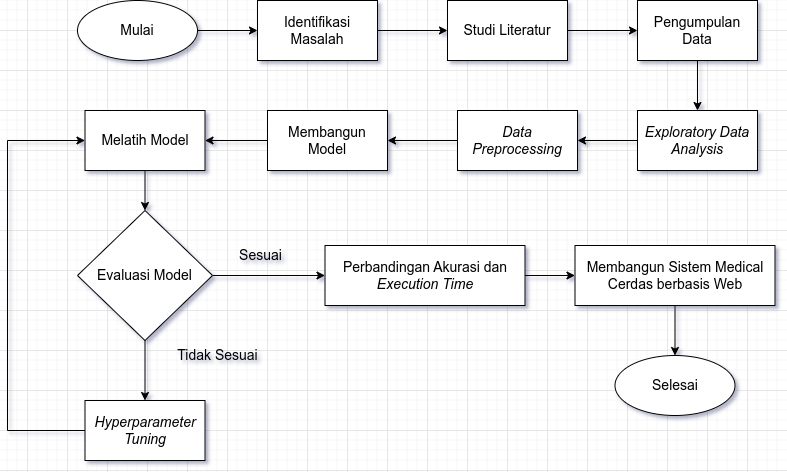
\includegraphics[width=\textwidth]{image/bab3/diagram_alir_penelitian.png}}
\caption{Diagram alir penelitian}
\label{alur_penelitian}
\end{figure}

\subsection{Identifikasi masalah}

\par Proses identifikasi masalah merupakan langkah awal dalam menentukan isu utama yang menjadi fokus penelitian ini. Tahapan ini mencakup penjabaran latar belakang masalah yang mendasari perlunya penelitian dilakukan. Selain itu, dirumuskan pertanyaan penelitian yang jelas untuk memandu arah penelitian, diikuti dengan penetapan tujuan penelitian yang ingin dicapai, dan diakhiri dengan manfaat yang diharapkan dari hasil penelitian.

\subsection{Studi literatur}

\par Tahap ini dilakukan dengan mengumpulkan dan memahami informasi terkait topik penelitian secara mendalam dari beberapa sumber. Referensi berkaitan dengan penelitian diambil dari buku, jurnal ilmiah, artikel, laporan penelitian, dan sumber relevan lainnya. Tujuan dari metode ini adalah untuk mendapatkan pemahaman yang mendalam tentang masalah beserta teori-teori yang mendukung penelitian.

\subsection{Pengumpulan data}
\par  Dataset dummy dibentuk dengan memperhatikan karakteristik pengguna e-learning. Fitur yang dipilih merepresentasikan pola penggunaan sistem. Contoh data misal dari Kaggle tentang ulasan pada \cite{pathi_imdb_movie_reviews}

\subsection{Pra-pemrosesan data}

\par Pra-pemrosesan data adalah serangkaian langkah krusial yang dilakukan sebelum data mentah digunakan untuk analisis atau pelatihan model machine learning. Proses ini bertujuan untuk membersihkan, mengubah, dan mempersiapkan data agar lebih akurat, konsisten, dan sesuai untuk tujuan analisis yang diinginkan. Data mentah seringkali mengandung kebisingan, nilai yang hilang (data \textit{missing values}), format yang tidak konsisten, atau \textit{outlier} yang dapat memengaruhi kinerja model secara signifikan. 

\begin{enumerate}
\item \textbf{Pembersihan data}: Menangani nilai yang hilang (misalnya dengan imputasi atau penghapusan baris), mengidentifikasi dan mengoreksi error atau ketidakakuratan, serta menghapus data duplikat.
   \item \textbf{Normalisasi data}: normaliasi data agar semua fitur memiliki skala yang sama.
   \item \textbf{Encoding label}: encoding label kategorikal (Kualitas) menjadi bentuk numerik.
   \item \textbf{Pemecahan dataset} : membagi menjadi data latih dan uji dengan rasio 80:20.
\end{enumerate}
 
\subsection{Melatih model}  

\par Pelatihan model menggunakan Algoritma KNN. Model dilatih menggunakan library Scikit-learn di Python dengan nilai k=5 . Tahap ini bertujuan untuk menemukan tetangga terdekat dari setiap data uji.

\subsection{Evaluasi model} 
\par Setelah model dilatih, data uji digunakan untuk mengukur kinerja model. Metrik evaluasi yang digunakan meliputi akurasi, presisi, recall, dan F1-score.


\subsection{Analisis hasil}
\par Hasil evaluasi dianalisis untuk mengetahui seberapa baik model dapat memprediksi kualitas pengguna. Selain itu, dilakukan analisis terhadap kelebihan dan keterbatasan metode KNN dalam konteks penelitian ini.

%-----------------------------------------------------------------------------%

% Baris ini digunakan untuk membantu dalam melakukan sitasi
% Karena diapit dengan comment, maka baris ini akan diabaikan
% oleh compiler LaTeX.
\begin{comment}
\bibliography{daftar-pustaka}
\end{comment}
